%% Chapter 1 --- Introduction (English version; labels match the Portuguese deposit version).
\chapter{Introduction}
\label{chap:introducao}

\section{Context and motivation}
\label{sec:intro-contexto}

``On tabular data, gradient boosting always wins.'' Few maxims of
machine-learning practice have been repeated as often over the last
decade, and, unlike most, this one even acquired a quantitative form: in
2022, a systematic study identified the inductive biases that explain
why tree ensembles beat neural networks on typical tables
\citep{grinsztajn2022}, and subsequent larger-scale evaluations nuanced
the verdict without overturning it \citep{mcelfresh2023}. For the
practitioner, the maxim became a decision shortcut: faced with a table,
use XGBoost and move on.

Consider, however, the concrete decision the maxim is meant to settle.
A data-science team must choose the model that will decide credit
approvals in production (a problem in the family of the
\texttt{credit\_g} and
\texttt{give\_\allowbreak me\_\allowbreak some\_\allowbreak credit}
datasets of this study), or the one that will estimate prices and
durations accompanied by prediction intervals, as in the real-estate
datasets \texttt{miami\_housing} and \texttt{kings\_county} used in the
distillation study (Chapter~\ref{chap:destilacao}). In 2026, that team
faces a menu the maxim never anticipated: besides the three
consolidated gradient-boosting implementations, there are a dozen deep
architectures claiming to have caught up, two Kolmogorov--Arnold
networks with strong claims of superiority and, at the center of
attention, tabular foundation models: pre-trained networks that
dispense with any task-specific training, because the training set
enters as context at prediction time \citep{hollmann2025,tabfm2026}.
Each proponent publishes numbers in its own favor, measured under
differing protocols, with differing tuning budgets and, increasingly,
without peer review. What the team lacks is evidence produced under a
single protocol and a procedure to turn it into a choice.

This dissertation produces both. The picture that emerges contradicts
the maxim on two counts. First, in the generation of models preceding
2026, the top of the accuracy ranking is a \emph{statistical tie}:
under a region of practical equivalence of one percentage point of
AUC, 8 of the 10 non-leading models are practically equivalent to the
leader --- itself already a foundation model, TabPFN, at average rank
3.2 --- under the lenient criterion (3 of the 10, the GBDTs, under the
strict 0.95 cutoff), and performance variance is dominated by the
model$\times$dataset interaction together with noise (the winner
depends on the dataset,
not on the family); ``boosting always wins'' finds no accuracy margin
to support it (Chapter~\ref{chap:benchmark}). Second, the 2026
generation shifts the top in an unexpected direction: what moved ahead
was not tuned deep learning but pre-training. TabFM, evaluated
zero-shot, with no tuning whatsoever, is the best model on \textbf{13
of the 18 datasets} of the benchmark and leads the average rank in all
three tasks (in multiclass, over the two datasets where it operates)
--- a lead that is consistent across datasets, which the tests,
underpowered with so few datasets per task, do not confirm as a
statistical separation (Chapter~\ref{chap:benchmark}). The price,
however, changes the nature of the decision: the accuracy leader costs
about \textbf{43 milliseconds per row} to serve predictions, against
\textbf{0.33 microseconds} for XGBoost --- amortized batch-serving
latencies, each model on its natural device (four to five orders of
magnitude; roughly 131~thousand times on the reference dataset, with
the ratio varying by dataset). The practical question becomes a
different one: does the leader's latency fit the use case and, if it
does not, what then?

That second question gives the dissertation its third line of work.
The obstacle to adopting the leader is an architectural cost (the
training set travels with the model on every prediction), and
architectural costs can, in principle, be transferred away: knowledge
distillation \citep{hinton2015} trains, on the expensive teacher's
outputs, a student that serves predictions in about a hundred
microseconds per row. For tabular foundation models, the literature established this
route for classification \citep{pocketfm2026}. What it transfers in
\emph{regression}, in particular when the preservation target is the
full predictive distribution, with quantiles and calibrated
intervals, had no academic answer as of the dated checks of this
study. The answer found is selective: \emph{point}
distillation fails robustly, \emph{distributional} distillation works
where the teacher has a genuine advantage, and the boundary between
the two conditions can be checked in minutes
(Chapter~\ref{chap:destilacao}).

\section{Research problem}
\label{sec:intro-problema}

The problem this dissertation confronts can be stated in three layers,
each inheriting the previous one. In the first layer there is a
\emph{vacuum of comparable evidence}: the families of tabular models
available in 2026 (gradient boosting; deep learning in its three
lineages --- dense networks, attention architectures, and
Kolmogorov--Arnold networks --- and in-context-learning foundation
models) had not been measured under a single protocol combining
hyperparameter selection strictly separated from measurement,
statistical inference able to \emph{affirm} equivalences rather than
only reject them, and cost axes (training time, tuning cost, and
serving latency) measured under the same conditions as accuracy. The
reference benchmarks predate the 2026 generation
\citep{grinsztajn2022,mcelfresh2023}, and that generation's numbers
came mostly from its own proponents.

In the second layer, even with the evidence produced, the problem of
\emph{decision} remains: benchmarks describe, but teams must choose.
The algorithm-selection literature suggests learning a router from
meta-features of the problem \citep{rice1976}; before recommending a
router, one must test whether it generalizes in the realistic regime
of a few dozen datasets, and the literature rarely reports that test.
Until it is confronted with data that played no part in its
construction, a decision artifact remains a hypothesis.

In the third layer, the evidence and the decision artifact point
together to a single operational obstacle: the latency of the new
accuracy leader. The problem then becomes one of science-driven
engineering: determining what knowledge distillation can and cannot
transfer from a tabular foundation model in regression, at what
serving cost, and under which conditions verifiable \emph{a priori}.
The central focus is distributional regression, the axis along which
the teacher carries information that the raw data do not hand to the
student.

\section{Objectives}
\label{sec:intro-objetivos}

\subsection{General objective}

To establish, under a single experimental protocol, with selection
separated from measurement and inference able to affirm equivalences,
the comparative evidence on the three families of tabular models in
the era of foundation models, and to convert it into evaluated
decision instruments (the learned component out of sample), including
the assessment, through knowledge distillation, of how far the
leading family's main operational obstacle can be removed.

\subsection{Specific objectives}

\begin{itemize}
  \item Run a multi-criteria benchmark of 14 models on 18 public
    OpenML datasets, with hyperparameter selection separated from
    measurement, an untouched hold-out, tuning budgets fixed per
    family (with the cost asymmetry measured and disclosed) and
    frequentist \emph{and} Bayesian statistical inference with a
    region of practical equivalence;
  \item Measure, under the same protocol, the cost axes the
    literature rarely reports (training time, total hyperparameter
    tuning cost and inference latency) and cross them with
    performance on Pareto frontiers;
  \item Include and adjudicate, with dated novelty checks, the two
    2026 additions: the neutral comparison between the two foundation
    models (TabPFN and TabFM) and the first independent test of the
    Kolmogorov--Arnold family against the full grid of families;
  \item Build a constraint-oriented decision framework, evaluate
    its learned component by leave-one-dataset-out and confront it
    with fixed policies (assessed descriptively) under a regret
    metric, including the
    extension to multi-criteria regret weighted by latency
    preferences;
  \item Characterize, through a pre-registered instance-level
    complementarity analysis, where foundation models and the best
    GBDT disagree --- and whether that disagreement is routable;
  \item Investigate what knowledge distillation transfers from
    tabular foundation models in regression, point and
    distributional; measure the frontier of serving strategies
    (distill, compress the context, shrink the ensemble) on the same
    hold-outs; test the distilled student against classical
    distributional baselines and measure the decision utility of the
    distributional gain in problem units, both in registered
    experiments; and condense the conditions of value into a
    practical decision rule;
  \item Ground all conclusions in reproducible infrastructure (fixed
    seeds, versions and data, versioned artifacts), under an explicit
    scientific-conduct contract (pre-registration of hypotheses,
    dated novelty checking, reporting of negative results and
    recorded correction of errors).
\end{itemize}

\section{Research questions}
\label{sec:intro-qps}

Three research questions organize the dissertation; each is answered
by one results chapter, and all three are revisited, with the
accumulated evidence, in the conclusion. The ``tie'' that RQ1 refers
to is the state of the literature immediately preceding this study:
large-scale evaluations report that, on a good share of tabular
datasets, the performance difference between gradient boosting and
tuned deep learning is small and the winner alternates with the
dataset \citep{mcelfresh2023}; the ``realistic'' $N$ of RQ2 is the
regime of a few dozen datasets in which any operational benchmark
lives.

\begin{description}
  \item[RQ1.] \emph{Does the accuracy tie among tabular model
    families survive a rigorous protocol (hold-out untouched by
    selection, Bayesian practical equivalence, cost axes) and the
    arrival of the 2026 generation of foundation models?}
    (Chapter~\ref{chap:benchmark})
  \item[RQ2.] \emph{Which decision artifact can a benchmark with a
    realistic $N$ of datasets actually support, a learned router or a
    constraint-based policy --- and how does that answer change when
    the decision weighs accuracy against cost?}
    (Chapter~\ref{chap:framework})
  \item[RQ3.] \emph{What does knowledge distillation transfer from a
    tabular foundation model in regression, at what serving cost, and
    under which conditions verifiable a priori?}
    (Chapter~\ref{chap:destilacao})
\end{description}

Figure~\ref{fig:intro-qps} summarizes the chain in which each
question's answer creates the next question: the tie and its shift
(RQ1) make the multi-criteria decision unavoidable (RQ2), and the
decision policy runs into a single obstacle, whose reduction is the
object of RQ3. The falsifiable hypotheses attached to the questions,
with their decision criteria, are stated where they are tested: in
the benchmark (Chapter~\ref{chap:benchmark}), in experiment E2
(Chapter~\ref{chap:framework}) and in the two-stage design of the
distillation study (Chapter~\ref{chap:destilacao}). In the diagram,
solid arrows link each question to the chapter that answers it, and
dashed arrows mark this logical chain; Chapters~\ref{chap:fundamentacao}
to~\ref{chap:metodologia} provide, respectively, the vocabulary, the
positioning in the literature and the protocol shared by the three
lines of work.

\begin{figure}[htb]
\centering
% Pre-compiled diagram (editable source: tikz-src/tikz-cap1-1-en.tex;
% recompile with: tectonic tikz-src/tikz-cap1-1-en.tex && mv tikz-cap1-1-en.pdf images/)
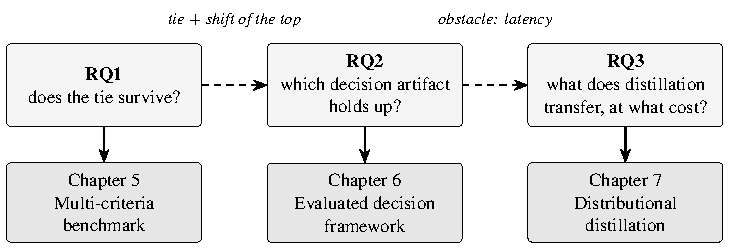
\includegraphics{images/tikz-cap1-1-en.pdf}
\caption[Research questions and chapters]{Research questions and the
chapters that answer them (the shift of the top is a consistent
lead, not a statistically confirmed separation). Source: the
author.}
\label{fig:intro-qps}
\end{figure}

\section{Summary of contributions}
\label{sec:intro-contribuicoes}

The contributions of this dissertation lie in measurement under a
uniform protocol and in openly reported evaluation --- out of sample
wherever something is learned. No new learning mechanism is claimed;
what is claimed, with dated novelty checks, is the framing and the
evidence that were missing. In order of presentation:

\begin{enumerate}
  \item \textbf{A multi-criteria benchmark of the foundation-model
    era} --- 14 models $\times$ 18 datasets (250 of the 252 cells;
    two disclosed structural exclusions), with a hold-out untouched
    by selection, frequentist and Bayesian inference and three cost
    axes under the same protocol. It yields the two facts that
    structure the dissertation: the statistical tie of the previous
    generation (8 of 10 models practically equivalent to the leader
    under the lenient criterion, 3 of 10 under the strict cutoff;
    rank variance dominated by the model$\times$dataset interaction
    together with noise)
    and the consistent lead of the 2026 generation (TabFM with the
    best rank in all three tasks and best model on 13 of 18
    datasets, zero-shot, without confirmation as a statistical
    separation by the underpowered tests, at the price of four to
    five orders of magnitude in latency). It includes the first
    neutral TabPFN~$\times$~TabFM comparison under an identical
    protocol, as far as the dated checks reach
    (Chapter~\ref{chap:benchmark}).
  \item \textbf{An independent negative result on Kolmogorov--Arnold
    networks.} In the first test of the family against the full
    GBDT (gradient-boosted decision trees)/deep
    learning/foundation-model grid in a multi-criteria benchmark
    (dated check), KAN and TabKAN finish in the bottom third on all
    three tasks, though cheap to serve: under a uniform protocol
    with tuning under paired conditions, the original papers' claims
    do not hold up (Chapter~\ref{chap:benchmark}).
  \item \textbf{A decision framework that is evaluated, not merely
    described.} Three studies evaluate the framework's components (the flowchart
    itself is their synthesis, not an evaluated policy) --- the
    learned component under leave-one-dataset-out: meta-feature
    routing does not generalize (hit rate 0.11 against 0.44 for the
    trivial baseline in the 11-model study; 0.72 against 0.78 with
    14); the fixed ``foundation model first'' policy is
    regret-optimal on the primary metric in a descriptive
    evaluation, with median regret of zero
    in the 2026 generation; and experiment E2 locates the inversion
    point (shifting 10 to 20\% of the weight from accuracy to
    latency, by median regret under the rank normalization adopted,
    is enough to flip
    the recommendation), quantitatively justifying the flowchart's
    architecture (Chapter~\ref{chap:framework}).
  \item \textbf{Distributional distillation of tabular foundation
    models.} On 20 regression datasets, under hypotheses registered
    before the experiments (Chapter~\ref{chap:destilacao}), it is
    shown that: (a) \emph{point} distillation does not work --- the
    student trained on the teacher's means beats the control on 4 of
    20 datasets with TabPFN, and the replication with TabFM as
    teacher, on the five central datasets, remains negative (a
    result reported with full prominence); (b) distilling the
    quantile curves works in part --- median retention of 12\% to
    19\% of the teacher's distributional advantage, depending on how
    the students are tuned, positive on 16 of 20 datasets (sign
    test, $p\approx0.019$ under the two-stage design correction);
    (c) the distilled student beats classical distributional
    baselines on 17 of 20 datasets (experiment E1); (d) distilling,
    compressing the context and shrinking the ensemble are measured
    on the same hold-outs, and out-of-fold labeling protects
    calibration, not accuracy; (e) these results condense into a
    decision rule whose precondition is measured in minutes. The
    dated searches of this study found no prior academic work on
    this framing (Chapter~\ref{chap:destilacao}).
  \item \textbf{Reusable infrastructure and conduct.} The protocol,
    the versioned artifacts (every number in the text traces to a
    CSV, JSON or executed notebook), the pre-registrations with
    dated addenda, the recorded novelty checks and the public
    error-correction procedure together constitute a methodological
    reproducibility contribution, described in
    Chapter~\ref{chap:metodologia} and exercised throughout the
    empirical part.
\end{enumerate}

\section{Publications}
\label{sec:intro-producao}

As of the submission of this dissertation, the research had produced
two technical reports of the graduate program, corresponding to its
individual-coursework requirements, both in English and available in
the project's public repository:

\begin{itemize}
  \item \textbf{AI-1} --- \emph{Does ``GBDT Always Win''? A
    Multi-Criteria Benchmark of 14 Tabular Models --- From a
    Statistical Tie to the 2026 Break --- and a Validated Decision
    Framework} \citep{companion2026}: technical report of the
    \emph{Trabalho Individual} (individual project) coursework
    (\texttt{latex/ai1/} in the repository), condensing the material of
    Chapters~\ref{chap:benchmark} and~\ref{chap:framework}.
  \item \textbf{AI-2} --- \emph{Distilling Tabular Foundation Models
    Beyond Classification: Distributional Regression and the
    Distill/Compress/Shrink Pareto Frontier}
    \citep{companion-ai2-2026}: technical report of the
    \emph{Atividade de Orientação Individual} (individual supervised
    research activity) (\texttt{latex/ai2/}), condensing the
    material of Chapter~\ref{chap:destilacao}; a preprint derived
    from it is being prepared for submission to arXiv.
\end{itemize}

Both reports are graded program coursework, without external peer
review as of this writing; their content corresponds, respectively,
to Chapters~\ref{chap:benchmark} and~\ref{chap:framework} and to
Chapter~\ref{chap:destilacao}, which additionally include three
contributions new to the dissertation: E2 (weighted multi-criteria
regret), entirely new relative to the reports; the complete
per-dataset results of E1 (the 17/20 paired comparison against
classical baselines; the distillation report incorporates the E1
data only through the five-system Friedman test); and the
instance-level complementarity analysis
(Section~\ref{sec:cap5-ato5}), pre-registered and executed after the
reports, which answers \emph{where} and \emph{in which cases}
foundation models beat GBDTs.

\section{How to read this dissertation}
\label{sec:intro-comoler}

The dissertation was written for three reader profiles, and not all
of them need to traverse it linearly. The \textbf{practitioner}, who
needs to choose and serve a tabular model, can go directly to
Chapters~\ref{chap:benchmark} and~\ref{chap:framework} (the evidence
and the decision flowchart) and to the decision rule that closes
Chapter~\ref{chap:destilacao} (Section~\ref{sec:destil-regra}): all
three were written to be self-contained, with the minimal
prerequisites recapped at the start of each chapter. The
\textbf{statistically minded reader} interested in the rigor of the
comparisons should start with Section~\ref{sec:fund-estatistica} of
Chapter~\ref{chap:fundamentacao} (the theory of the tests, including
the Bayesian practical-equivalence layer) and with
Chapter~\ref{chap:metodologia} (the application protocol, the policy
for missing cells and the limitations disclosed before the results).
The \textbf{replicator}, who wants to reproduce or extend the
experiments, finds in Chapter~\ref{chap:metodologia} the complete
protocol with seeds, versions and justifications, and in the
appendices the rest: the complete per-dataset tables
(Appendix~\ref{app:tabelas}), the hyperparameter search spaces
(Appendix~\ref{app:espacos-busca}) and the supplementary results and
ablations; every artifact cited has an explicit path in the
project's public repository.

\section{Structure of the dissertation}
\label{sec:intro-estrutura}

The remainder of the dissertation is organized into seven chapters
and three appendices. \textbf{Chapter~\ref{chap:fundamentacao}}
builds, from the concrete to the abstract, the technical vocabulary
of the work: tabular data and their constitutive heterogeneity,
trees and gradient boosting, the three lineages of tabular deep
learning, foundation models and the in-context-learning mechanism,
knowledge distillation, the toolkit of distributional regression
(quantiles, CRPS, calibration), the theory of statistical tests for
algorithm comparison and the decision vocabulary (algorithm
selection, regret, Pareto dominance), each at a depth proportional
to the use the later chapters make of it.
\textbf{Chapter~\ref{chap:related}} positions the work along six
axes of the literature, from tabular benchmarks to the distillation
of foundation models, closing with a synthesis table that links each
gap, characterized by dated online checks, to the chapter that
attacks it. \textbf{Chapter~\ref{chap:metodologia}} specifies the
experimental protocol shared by the whole empirical part: datasets,
models, internal selection with an untouched hold-out, metrics, the
statistical-inference protocol, cost measurement, reproducibility
infrastructure and the scientific-conduct contract, with the
design's limitations disclosed before any result.
\textbf{Chapter~\ref{chap:benchmark}} presents the benchmark in five
acts (the statistical tie of the 11-model core, the cost axes on
which the tied models differ by orders of magnitude, the conditional
reversals and the sample-size axis, the shift of the top by the 2026
generation --- a consistent lead, without confirmation as a
statistical separation --- together with the negative result on
Kolmogorov--Arnold networks, and the instance-level complementarity
between foundation models and GBDTs), answering RQ1.
\textbf{Chapter~\ref{chap:framework}} submits the decision framework
to three studies (the negative result of meta-feature routing, this
one under leave-one-dataset-out; the descriptive evaluation of the
``foundation model first'' policy; and the registered experiment on
weighted multi-criteria regret), consolidating the four-constraint
flowchart that answers RQ2. \textbf{Chapter~\ref{chap:destilacao}}
presents the distributional-distillation contribution under a
registered two-stage design: the refutation of point distillation,
the success of quantile-curve transfer, the frontier of three
serving strategies, the out-of-fold labeling ablation, experiment E1
against classical baselines and the final decision rule that answers
RQ3. \textbf{Chapter~\ref{chap:conclusao}} confronts each research
question with the accumulated evidence, consolidates the
contributions, discloses the limitations and threats to validity of
the program as a whole and points to future work. The
\textbf{appendices} gather the complete per-dataset result tables,
the hyperparameter search spaces and the supplementary results and
ablations.
